\documentclass{beamer}
\usetheme{default}

\usepackage{graphicx}
\graphicspath{{../../images/}}

\setbeamertemplate{caption}[numbered]

\title{Chapter-02: Client-Server Architecture}
\subtitle{IF231303-Software Architecture\\Pradita University}
\author{Alfa Yohannis}
\begin{document}

\begin{frame}[plain]
    \maketitle
\end{frame}

\begin{frame}{Background}
\begin{itemize}
\item Computer started as a single unit.  Software only ran on that single unit.
\item The singular systems then gradually separated into different units, .i.e., for data storage and processing.
\item Certain functionalities tend to grow overtime and require separate machines.
\item Computer networking then became common. Different nodes can exchange messages with each other.
\item Each node may have different roles.
\item Distributed systems then appear.
\end{itemize}
\end{frame}

\begin{frame}{Client-Server}
\begin{itemize}
\item A client-server environment consists of, at least, a server and one or more clients.
\item The server usually has more computing power than the clients. 
\item It receives request from the clients to perform certain tasks and then returns the results.
\item Two-tier Architecture:
\begin{itemize}
\item Desktop apps + database server
\item Browser + web server
\end{itemize}
\item Three-tier Architecture:
\begin{itemize}
\item Browser + application/web server + database server
\end{itemize}
\end{itemize}
\end{frame}

\begin{frame}{Advantages}
\begin{itemize}
\item Computation can be accessed by multiple nodes/users from different remote locations.
\item High-performance computation can be delegated to the server.
\item Data can be centralised and therefore reduce data duplication.
\item Scalable:
\begin{itemize}
\item Vertical scaling (upgrading a machine's specs)
\item Horizontal scaling (adding more nodes/machines)
\end{itemize}
\end{itemize}
\end{frame}

\begin{frame}{Disadvantages}
\begin{itemize}
\item More complex to manage:
\begin{itemize}
\item Cost (more components/machines to manage)
\item Security (it operates in a network, prone to cyber attack)
\item Coordination (e.g., async, sync, parallelism)
\item Compatibility (e.g., different clients' specs)
\item Network problems (e.g., latency)
\end{itemize}
\end{itemize}
\end{frame}

\begin{frame}{Schema}
\begin{figure}[h]
    \centering
    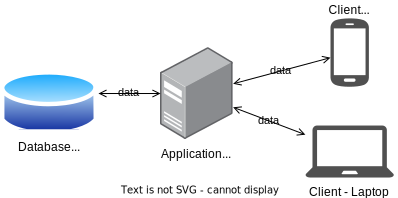
\includegraphics[width=\textwidth]{client-server-3-tier}
    \caption{3-tier client-server architecture.}
    \label{fig:client-server-schema}
\end{figure}
\end{frame}

\end{document}
